\chapter{Introduction}
\markright{Introduction}
\label{ChapterOne}
\section{Reading Instructions}
\label{sec:Reading Instructions}
\indent This thesis may present different interests for different readers. In this chapter, I will provide a guideline explaining what is covered in each chapter in order to facilitate browsing of the thesis and efficiently help every reader find the relevant information for him/her. 

\indent The first chapter presents the details and circumstances in which this thesis was created upon. The Problem statement of this thesis will be defined along with the motivation for solving that specific problem. Readers interested in a high level overview of the goal and the approach used for solving the specified problem, along with the original contribution brought to the existing system should refer to the \textit{GoalAndApproach} and \textit{OriginalContribution} sub chapters respectively.

\indent The second chapter will discuss the most relevant concept of this thesis, namely decision support systems. They will be discussed and evaluated in terms of the foundations they are built on, their functionality, the Interfaces used for them, how they are implemented and their evaluation matrices and impact on decisions. This chapter will be most relevant for readers who would like to learn about decision support systems and understand the underlying concepts.

\indent The third chapter will cover the Connect Hydro Project that my thesis aims to support and add to it. Connect Hydro proposes a system to connect small, private and independent hydro power plants through networked intelligent control system. In the chapter, I will also give an overview on the device they developed to collect sensor data from the power plants.

\indent Chapter four will highlight in detail how a decision support system can bring advantage to the connect hydro project. In this chapter, I will also discuss what are the requirements for this proposed decision support system and describe the different inputs along with the expected outputs in addition to what should be the defined rules for such system. This is the chapter that my work will be based on.

\indent The fifth chapter will cover the technical aspects of the implementation done to support this thesis. It will begin with describing the frameworks and technologies used for the implementation while explaining why they were used. Furthermore, each implemented aspect of the project will be explained in detail, namely the database model, the web portal, the data visualization and finally and most importantly the decision support system. This chapter might be of interest also for readers that want to find more details about the design and implementation of this system.

\indent Chapter six will explain how the system implemented was evaluated, what matrices were used in its evaluation and the results. Readers interested in the results only will find this chapter the most informative for them.

\indent The last chapter containing the conclusion and the future research will be most relevant for users interested in extending and improving the proposed system.
\section{Foreword}
\label{sec:Foreword}
Conventional energy sources based on oil, coal, and natural gas have proven to be highly effective drivers of economic progress especially with increasing improvements in the quality of life, industrialization of developing nations, and increase of the world population. However, this excessive fossil fuel consumption not only leads to an increase in the rate of diminishing fossil fuel reserves, but it also has a significant adverse impact on the environment, resulting in increased health risks and the threat of global climate change \cite{herzog2001renewable}. These traditional fossil fuel-based energy sources are facing increasing pressure on several environmental fronts. The increasing consumption of fossil fuel to meet the current energy demands causes alarm over the energy crisis and has generated a lot of interest in promoting renewable alternatives to meet the developing world's growing energy needs \cite{youm2000renewable,hiemstra2009fuelwood}. Excessive use of fossil fuels has caused global warming by carbon dioxide; therefore, renewable promotion of clean energy is required \cite{hall1991cooling}. An agreement called "Kyoto Protocol agreement" was made  with the objective of monitoring the greenhouse emissions with an overall pollution prevention target \cite{panwar2011role}. Due to these facts, Research is directed towards utilizing already available renewable energy sources(RES) as well as finding new sources. 

Renewable energy is energy that is generated from natural processes that are continuously replenished. This energy cannot be exhausted and can be used to provide sustainable energy services, based on the use of routinely available, indigenous resources. There is an enormous potential of renewable energy sources as they can in principle meet many times the world’s energy demand \cite{herzog2001renewable}. It is becoming increasingly likely to transition to renewable-based energy systems like solar, wind or hydro power systems. Fossil fuel and renewable energy prices, social and environmental costs are heading in opposite directions. The cost of implementing renewable-based systems have dropped significantly in the past 30 years and continue to drop, while the price of oil and gas (Fossil fuel) continue to fluctuate \cite{herzog2001renewable}. Society is slowly moving towards seeking more sustainable production methods, waste minimization, reduced air pollution from vehicles, distributed energy generation, conservation of native forests, and reduction of greenhouse gas emissions. Changes towards environmental improvements are becoming more politically acceptable globally, especially in developed countries. 

Renewable energy sources currently supply somewhere between 14\% of world’s total energy demand \cite{panwar2011role}. The supply is dominated by traditional biomass, mostly fuel wood used for cooking and heating, especially in developing countries in Africa, Asia and Latin America \cite{herzog2001renewable}. Large hydro power stations are considered a major contributer; with nearly 20 percent of the global electricity supply by them \cite{panwar2011role}. New renewable energy sources (solar energy, wind energy, modern bio-energy, geothermal energy, and small hydro power) are currently contributing about two percent. A number of scenario studies have investigated the potential contribution of renewables to global energy supplies, indicating that in the second half of the 21st century their contribution might range from the present figure of nearly 20 percent to more than 50 percent with the right policies in place \cite{panwar2011role}. RESs are also called alternative energy sources. The share of RESs is expected to increase very significantly (30–80\% in 2100) \cite{fridleifsson2001geothermal}. Figure 1.1 shows the expected percentage for every type of renewable energy source currently and what they are expected to reach in 2040.
\begin{figure}[H]
\centering
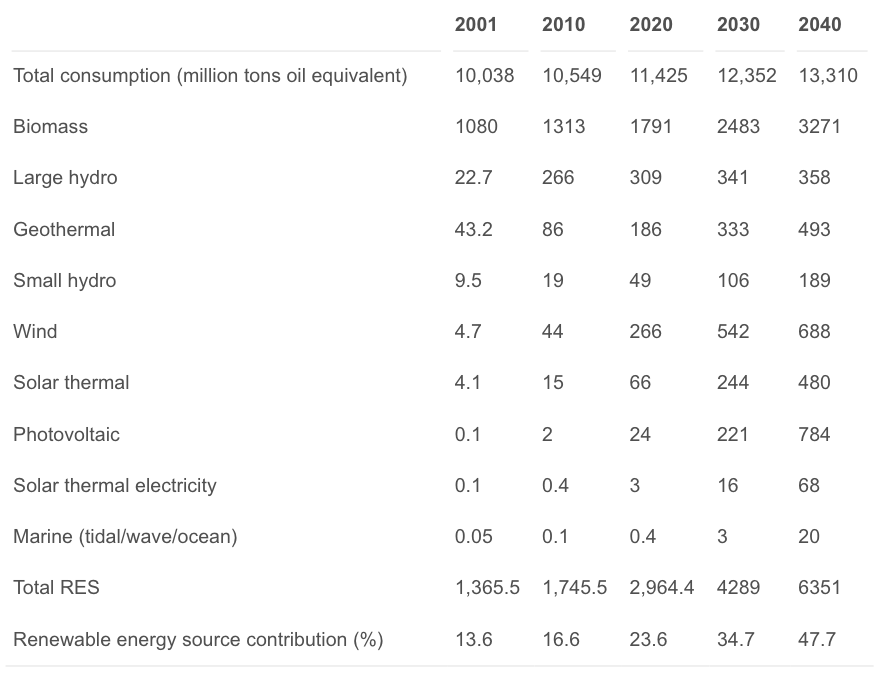
\includegraphics[scale=0.4]{Images/Percentage_of_Renewable_Sources.png}
\caption[Global renewable energy scenario by 2040]{Global renewable energy scenario by 2040 \cite{panwar2011role}}
\end{figure}
\subsection{Types of Renewable Energy Sources}
There exists different types of renewable energy sources. In this section we will discuss how each of them is harnessed and the different usages for the energy they produce.
\begin{itemize}
	\item \textbf{Solar Power:} It is the energy coming from sunlight. It can be exist in two different ways. The First is solar-thermal power which is harnessed using mirrors or lenses to concentrate a large area of sunlight, or solar thermal energy (STE), onto a small area (i.e. a solar cell) which is then used for heating or domestic use. The second way involves solar cells (usually made from slices of crystalline silicon) that rely on the photovoltaic (PV) effect to absorb photons and convert them into electrons. Solar power is one of the most popular, and fast growing, sources of alternative energy.
	\item \textbf{Wind Power:} It is the use of air flow through wind turbines to mechanically power generators for electric power. It is considered very reliable and steady, as wind is consistent from year to year and does not diminish during peak hours of demand. Wind energy can be used to pump water or generate electricity, but it has a huge startup construction cost for constructing a wind farm.
	\item \textbf{Hydroelectric energy:} The kinetic energy of flowing rivers is captured and converted into hydroelectricity. It involves the usage of flowing water to turn turbines that in turn generate electricity. It is one of the renewable energy forms with the highest potential due to the availability of its creating resource; the water.
	\item \textbf{Bio energy:} This is the use of plant matter and animal waste to create electricity. When converted properly, it is a low-carbon source of energy with little pollution. Some of the more modern forms of biomass energy are methane generation and production of alcohol for automobile fuel and fueling electric power plants. It is very expensive as it has not advanced as quickly as other forms of renewable energy sources.
	\item \textbf{Geothermal power:} It is energy derived from the heat of the earth itself. This heat can be sourced close to the surface or from heated rock and reservoirs of hot water miles beneath our feet. Geothermal power plants harness these heat sources to generate electricity. On a much smaller scale, a geothermal heat pump system can leverage the constant temperature of the ground found just ten feet under the surface to help supply heat to a nearby building in the winter, or help cool it in the summer.
	\item \textbf{Tidal Power:} It is considered to be a potential source of renewable energy because tides are steady and predictable. Tidal power suffers from relatively high cost and limited availability of sites with sufficiently high tidal ranges or flow velocities which makes its applications limited.
\end{itemize}
 The figure below explains the main usage of the different Renewable Energy sources. For Example: Hydro power is used for power generation, Solar power can be used for powering home appliances etc.
\begin{figure}[H]
\centering
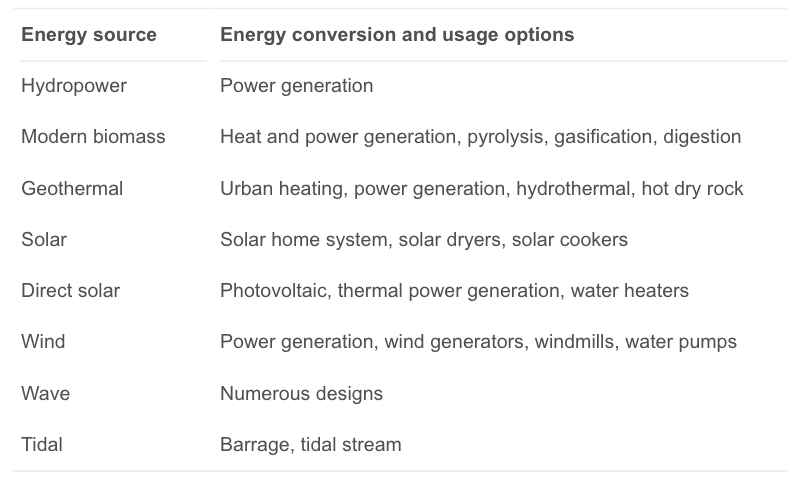
\includegraphics[scale=0.4]{Images/Types_of_Renewable_Sources.png}
\caption[Main renewable energy sources and their usage form]{Main renewable energy sources and their usage form \cite{panwar2011role}}
\end{figure}
\section{Motivation}          
\label{sec:Motivation}
Renewable energy is the new trend that all governments are directing research into, simply because they are environment friendly and cheap. All researchers predict that the earth natural resources will run out and for the past 20 years have been trying to research new techniques to produce energy \cite{SEIT2017}.

Small hydro power plants have a huge, untapped potential in most areas of the world and can make a significant contribution to future energy needs. It is largely dependent on already proven and developed technology. It has a considerable scope for development and optimization. In Austria, 9\% of its power demand is supplied from small hydro power stations. They are of great significance for the security of supply and regional economy due to their decentralized character \cite{SEIT2017}. The current trend is that electricity trading prices are constantly going down and the government is directing research towards finding alternative energy and utilizing the already available ones.
\section{Problem Statement}
\label{sec:Problem Statement}
In countries, where many small rivers exist, the geography can be used to implement environment-friendly small hydro power plants for the generation of energy. The smaller such hydro power plants are, the higher is the impact of environmental incidents. Usually, there are more than one small hydro power plants located alongside one river, mostly operated by different owners. For more than 100 years electricity is being produced by hydro power plants on the Alm river in Upper Austria. Today 55 small and micro hydro power plants of more than 40 owners are operated on 48 kilometers \cite{SEIT2017}. To increase the overall power generating efficiency of all hydro power plants alongside the river, a good communication- and cooperating concept is needed.

The lack of good communication and cooperating is creating a problem leading to less efficient energy production, higher down time for the power plants and more maintenance. The problem can be broken into different aspects. The first would be collecting the sensor data from the different power plants; given that each power plant uses different equipment; a method should be developed to collect these data and uniform them. The second aspect would be to use the data to help the power plant owners make informed decisions, this will lead to efficient energy production and less down time. The third aspect would be to perform the actions directly on the power plants instead of informing the owner to do them, this will result in a fully automated system that doesn't need any human interaction.

In this thesis, we will tackle the second phase. We will work under the assumption that the data is collected and unified. The aim is to provide the owners with informed decisions on how to operate their power plants. A formal description of our thesis problem is defined as follows: "Given sensor data from small, private \& independent hydro power plants, find decisions using the data coming from their sensors and external sources, such that the overall energy production is increased and the down time is minimized." 
\section{Goal and Approach}
\label{sec:GoalAndApproach}
As mentioned in the previous section, our goal is to provide the owners of small hydro power plants with informed decision based on the sensor data collected from all the power plants such that the overall energy production is increased and the down time is minimized. In order to solve the problem specified, we propose a system prototype implementation of a decision support system for several small, private and independent hydro power plants. This system should be able to manage general events that could occur and affect all power plants as well as handle specific rules defined for every power plant by the owner.

The focus of this thesis will be split into two parts. The first is performing sound research on decision support systems, their types and techniques and processes used to develop them. The second part is implementing a web portal with an embedded simple decision support system. The Decision support system should be a combination of a knowledge-driven and data-driven DSS. The second part should include a proposed database schema for the power plants sensor data as well.
\section{Original Contribution}
\label{sec:OriginalContribution}
Currently there exists no system connecting small hydro power plants. Owners of said power plants don't communicate with each other resulting in a need for an early warning system (Decision support system). The main goal of the Decision support system is to receive data from previous power plants along the same river and direct the owner to do some action in response to the data received.

In this thesis, a proof of concept will be developed to prove that a decision support can help small hydro power plants work efficiently and in synchronization with their neighbors to optimize their energy production. We will investigate the advantages of combining different decision support techniques to achieve the main goal as well as providing a simple prototype that can be used as a base for future research.
\section{Outline of the Thesis}
\label{sec:OutlineOfTheThesis}
The first chapter of the thesis makes a brief presentation of the concepts related with the project and makes the reader familiar with the aims and reasons that justify the selection of this topic. The background of the problem and a short description of the social and economic context are given in order to integrate the problem into the real world.

\indent The second chapter will discuss the concept of Decision support systems. It will investigate the foundations they are built on, their functionality, the Interfaces used for them, how they are implemented and their evaluation matrices and impact on decisions.

\indent The third chapter will cover the Small hydro power stations as well as the Connect Hydro Project. Small hydro power stations will be discussed in terms of their different types, advantages and disadvantages. Secondly, we will discuss the different control strategies that can be used to control small hydro power plants. Finally the Connect Hydro project will be introduced and the work related to it will be discussed.

\indent Chapter four will highlight in detail how a decision support system can bring advantage to the connect hydro project and how the prototype system was implemented and using which techniques.

\indent The fifth chapter will cover the technical aspects of the implementation done to support this thesis. It will begin with describing the frameworks and technologies used for the implementation while explaining why they were used. Furthermore, each implemented aspect of the project will be explained in detail, namely the database model, the web portal, the data visualization and finally and most importantly the decision support system.

\indent Chapter six will explain how the prototype implemented was evaluated, what matrices were used in its evaluation and the results.

\indent The last chapter contains the conclusion and the future research that can help in improving the proposed system.